% Options for packages loaded elsewhere
\PassOptionsToPackage{unicode}{hyperref}
\PassOptionsToPackage{hyphens}{url}
\PassOptionsToPackage{dvipsnames,svgnames,x11names}{xcolor}
%
\documentclass[
  authoryear,
  preprint,
  1p]{elsarticle}

\usepackage{amsmath,amssymb}
\usepackage{iftex}
\ifPDFTeX
  \usepackage[T1]{fontenc}
  \usepackage[utf8]{inputenc}
  \usepackage{textcomp} % provide euro and other symbols
\else % if luatex or xetex
  \usepackage{unicode-math}
  \defaultfontfeatures{Scale=MatchLowercase}
  \defaultfontfeatures[\rmfamily]{Ligatures=TeX,Scale=1}
\fi
\usepackage{lmodern}
\ifPDFTeX\else  
    % xetex/luatex font selection
\fi
% Use upquote if available, for straight quotes in verbatim environments
\IfFileExists{upquote.sty}{\usepackage{upquote}}{}
\IfFileExists{microtype.sty}{% use microtype if available
  \usepackage[]{microtype}
  \UseMicrotypeSet[protrusion]{basicmath} % disable protrusion for tt fonts
}{}
\makeatletter
\@ifundefined{KOMAClassName}{% if non-KOMA class
  \IfFileExists{parskip.sty}{%
    \usepackage{parskip}
  }{% else
    \setlength{\parindent}{0pt}
    \setlength{\parskip}{6pt plus 2pt minus 1pt}}
}{% if KOMA class
  \KOMAoptions{parskip=half}}
\makeatother
\usepackage{xcolor}
\setlength{\emergencystretch}{3em} % prevent overfull lines
\setcounter{secnumdepth}{5}
% Make \paragraph and \subparagraph free-standing
\makeatletter
\ifx\paragraph\undefined\else
  \let\oldparagraph\paragraph
  \renewcommand{\paragraph}{
    \@ifstar
      \xxxParagraphStar
      \xxxParagraphNoStar
  }
  \newcommand{\xxxParagraphStar}[1]{\oldparagraph*{#1}\mbox{}}
  \newcommand{\xxxParagraphNoStar}[1]{\oldparagraph{#1}\mbox{}}
\fi
\ifx\subparagraph\undefined\else
  \let\oldsubparagraph\subparagraph
  \renewcommand{\subparagraph}{
    \@ifstar
      \xxxSubParagraphStar
      \xxxSubParagraphNoStar
  }
  \newcommand{\xxxSubParagraphStar}[1]{\oldsubparagraph*{#1}\mbox{}}
  \newcommand{\xxxSubParagraphNoStar}[1]{\oldsubparagraph{#1}\mbox{}}
\fi
\makeatother


\providecommand{\tightlist}{%
  \setlength{\itemsep}{0pt}\setlength{\parskip}{0pt}}\usepackage{longtable,booktabs,array}
\usepackage{calc} % for calculating minipage widths
% Correct order of tables after \paragraph or \subparagraph
\usepackage{etoolbox}
\makeatletter
\patchcmd\longtable{\par}{\if@noskipsec\mbox{}\fi\par}{}{}
\makeatother
% Allow footnotes in longtable head/foot
\IfFileExists{footnotehyper.sty}{\usepackage{footnotehyper}}{\usepackage{footnote}}
\makesavenoteenv{longtable}
\usepackage{graphicx}
\makeatletter
\newsavebox\pandoc@box
\newcommand*\pandocbounded[1]{% scales image to fit in text height/width
  \sbox\pandoc@box{#1}%
  \Gscale@div\@tempa{\textheight}{\dimexpr\ht\pandoc@box+\dp\pandoc@box\relax}%
  \Gscale@div\@tempb{\linewidth}{\wd\pandoc@box}%
  \ifdim\@tempb\p@<\@tempa\p@\let\@tempa\@tempb\fi% select the smaller of both
  \ifdim\@tempa\p@<\p@\scalebox{\@tempa}{\usebox\pandoc@box}%
  \else\usebox{\pandoc@box}%
  \fi%
}
% Set default figure placement to htbp
\def\fps@figure{htbp}
\makeatother

\makeatletter
\@ifpackageloaded{caption}{}{\usepackage{caption}}
\AtBeginDocument{%
\ifdefined\contentsname
  \renewcommand*\contentsname{Table of contents}
\else
  \newcommand\contentsname{Table of contents}
\fi
\ifdefined\listfigurename
  \renewcommand*\listfigurename{List of Figures}
\else
  \newcommand\listfigurename{List of Figures}
\fi
\ifdefined\listtablename
  \renewcommand*\listtablename{List of Tables}
\else
  \newcommand\listtablename{List of Tables}
\fi
\ifdefined\figurename
  \renewcommand*\figurename{Figure}
\else
  \newcommand\figurename{Figure}
\fi
\ifdefined\tablename
  \renewcommand*\tablename{Table}
\else
  \newcommand\tablename{Table}
\fi
}
\@ifpackageloaded{float}{}{\usepackage{float}}
\floatstyle{ruled}
\@ifundefined{c@chapter}{\newfloat{codelisting}{h}{lop}}{\newfloat{codelisting}{h}{lop}[chapter]}
\floatname{codelisting}{Listing}
\newcommand*\listoflistings{\listof{codelisting}{List of Listings}}
\makeatother
\makeatletter
\makeatother
\makeatletter
\@ifpackageloaded{caption}{}{\usepackage{caption}}
\@ifpackageloaded{subcaption}{}{\usepackage{subcaption}}
\makeatother
\journal{Psychometrika}

\usepackage[]{natbib}
\bibliographystyle{elsarticle-harv}
\usepackage{bookmark}

\IfFileExists{xurl.sty}{\usepackage{xurl}}{} % add URL line breaks if available
\urlstyle{same} % disable monospaced font for URLs
\hypersetup{
  pdftitle={Let's talk about Thurstone \& Co.: An information-theoretical model for comparative judgments, and its statistical translation},
  pdfauthor={Jose Manuel Rivera Espejo; Tine van van Daal; Sven De De Maeyer; Steven Gillis},
  pdfkeywords={Probability, Directed Acyclic Graphs, Bayesian
methods, Thurstonian model, Comparative judgement, Structural Causal
Models, Statistical modeling},
  colorlinks=true,
  linkcolor={blue},
  filecolor={Maroon},
  citecolor={Blue},
  urlcolor={Blue},
  pdfcreator={LaTeX via pandoc}}


\setlength{\parindent}{6pt}
\begin{document}

\begin{frontmatter}
\title{Let's talk about Thurstone \& Co.: An information-theoretical
model for comparative judgments, and its statistical translation}
\author[1]{Jose Manuel Rivera Espejo%
\corref{cor1}%
}
 \ead{JoseManuel.RiveraEspejo@uantwerpen.be} 
\author[1]{Tine van Daal%
%
}
 \ead{tine.vandaal@uantwerpen.be} 
\author[1]{Sven De Maeyer%
%
}
 \ead{sven.demaeyer@uantwerpen.be} 
\author[2]{Steven Gillis%
%
}
 \ead{steven.gillis@uantwerpen.be} 

\affiliation[1]{organization={University of Antwerp, Training and
education sciences},,postcodesep={}}
\affiliation[2]{organization={University of
Antwerp, Linguistics},,postcodesep={}}

\cortext[cor1]{Corresponding author}




        
\begin{abstract}
(to do)
\end{abstract}





\begin{keyword}
    Probability \sep Directed Acyclic Graphs \sep Bayesian
methods \sep Thurstonian model \sep Comparative
judgement \sep Structural Causal Models \sep 
    Statistical modeling
\end{keyword}
\end{frontmatter}
    

\section{Introduction}\label{sec-introduction}

In \emph{comparative judgment} (CJ) studies, judges assess a specific
trait or attribute across various stimuli by performing pairwise
comparisons \citep{Thurstone_1927a, Thurstone_1927b}. Each comparison
produces a dichotomous outcome, indicating which stimulus is perceived
to exhibit a higher trait level. For example, when assessing text
quality, judges compare pairs of written texts (the stimuli) to
determine the relative quality each text exhibit (the trait)
\citep{Laming_2004, Pollitt_2012b, Whitehouse_2012, vanDaal_et_al_2016, Lesterhuis_2018_thesis, Coertjens_et_al_2017, Goossens_et_al_2018, Bouwer_et_al_2023}.

Numerous studies have documented the effectiveness of CJ in assessing
traits and competencies over the past decade. These studies have
emphasized three aspects of the method's effectiveness: its reliability,
validity, and practical applicability. Research on reliability indicates
that CJ requires a relatively small number of pairwise comparisons
\citep{Verhavert_et_al_2019, Crompvoets_et_al_2022} to produce trait
scores that are as precise and consistent as those generated by other
assessment methods
\citep{Coertjens_et_al_2017, Goossens_et_al_2018, Bouwer_et_al_2023}.
Furthermore, evidence suggests that the reliability and time efficiency
of CJ are comparable, if not superior, to those of other assessment
methods when employing adaptive comparison algorithms
\citep{Pollitt_2012b, Verhavert_et_al_2022, Mikhailiuk_et_al_2021}.
Meanwhile, research on validity suggests that scores generated by CJ can
accurately represent the traits under measurement
\citep{Whitehouse_2012, vanDaal_et_al_2016, Lesterhuis_2018_thesis, Bartholomew_et_al_2018, Bouwer_et_al_2023},
while research on practical applicability highlights the method's
versatility across both educational and non-educational contexts
\citep{Kimbell_2012, Jones_et_al_2015, Bartholomew_et_al_2018, Jones_et_al_2019, Marshall_et_al_2020, Bartholomew_et_al_2020, Boonen_et_al_2020}.

Nevertheless, despite the increasing number of CJ studies, unsystematic
and fragmented research approaches have left several critical issues
unaddressed. The present study primarily focuses on two: the
overreliance on the assumptions of Thurstone's Case V in the statistical
analysis of CJ data, and the apparent disconnect between CJ's approach
to trait measurement and hypothesis testing. The following sections
begin with a brief overview of Thurstone's theory and a detailed
examination of these issues. Subsequently, the study introduces a
theoretical model for CJ that builds upon Thurstone's theory, alongside
its statistical translation, designed to address the two concerns
simultaneously.

\section{Thurstone's theory}\label{sec-thurstone_theory}

In its most general form, Thurstone's theory addresses pairwise
comparisons where a single judge evaluates multiple stimuli
\citep[pp.~267]{Thurstone_1927b}. The theory posits that two key factors
determine the dichotomous outcome of these comparisons: the discriminal
process of each stimulus and their discriminal difference. The
\emph{discriminal process} captures the psychological impact each
stimulus exerts on the judge or, more simply, his perception of the
stimulus trait. The theory assumes that the discriminal process for any
given stimulus forms a Normal distribution along the trait continuum
\citep[pp.~266]{Thurstone_1927b}. The mode (mean) of this distribution,
known as the \emph{modal discriminal process}, indicates the stimulus
position on this continuum, while its dispersion, referred to as the
\emph{discriminal dispersion}, reflects variability in the perceived
trait of the stimulus.

Figure~\ref{fig-discriminal_process} illustrates hypothetical
discriminal processes along a quality trait continuum for two written
texts. The figure indicates that the modal discriminal process for Text
B is positioned further along the continuum than that of Text A
\((S_{B} > S_{A})\), suggesting that Text B exhibits higher quality.
Additionally, the figure highlights that Text B has a broader
distribution compared to Text A, which arises from its larger
discriminal dispersion \((\sigma_{B} > \sigma_{A})\).

\begin{figure}

\centering{

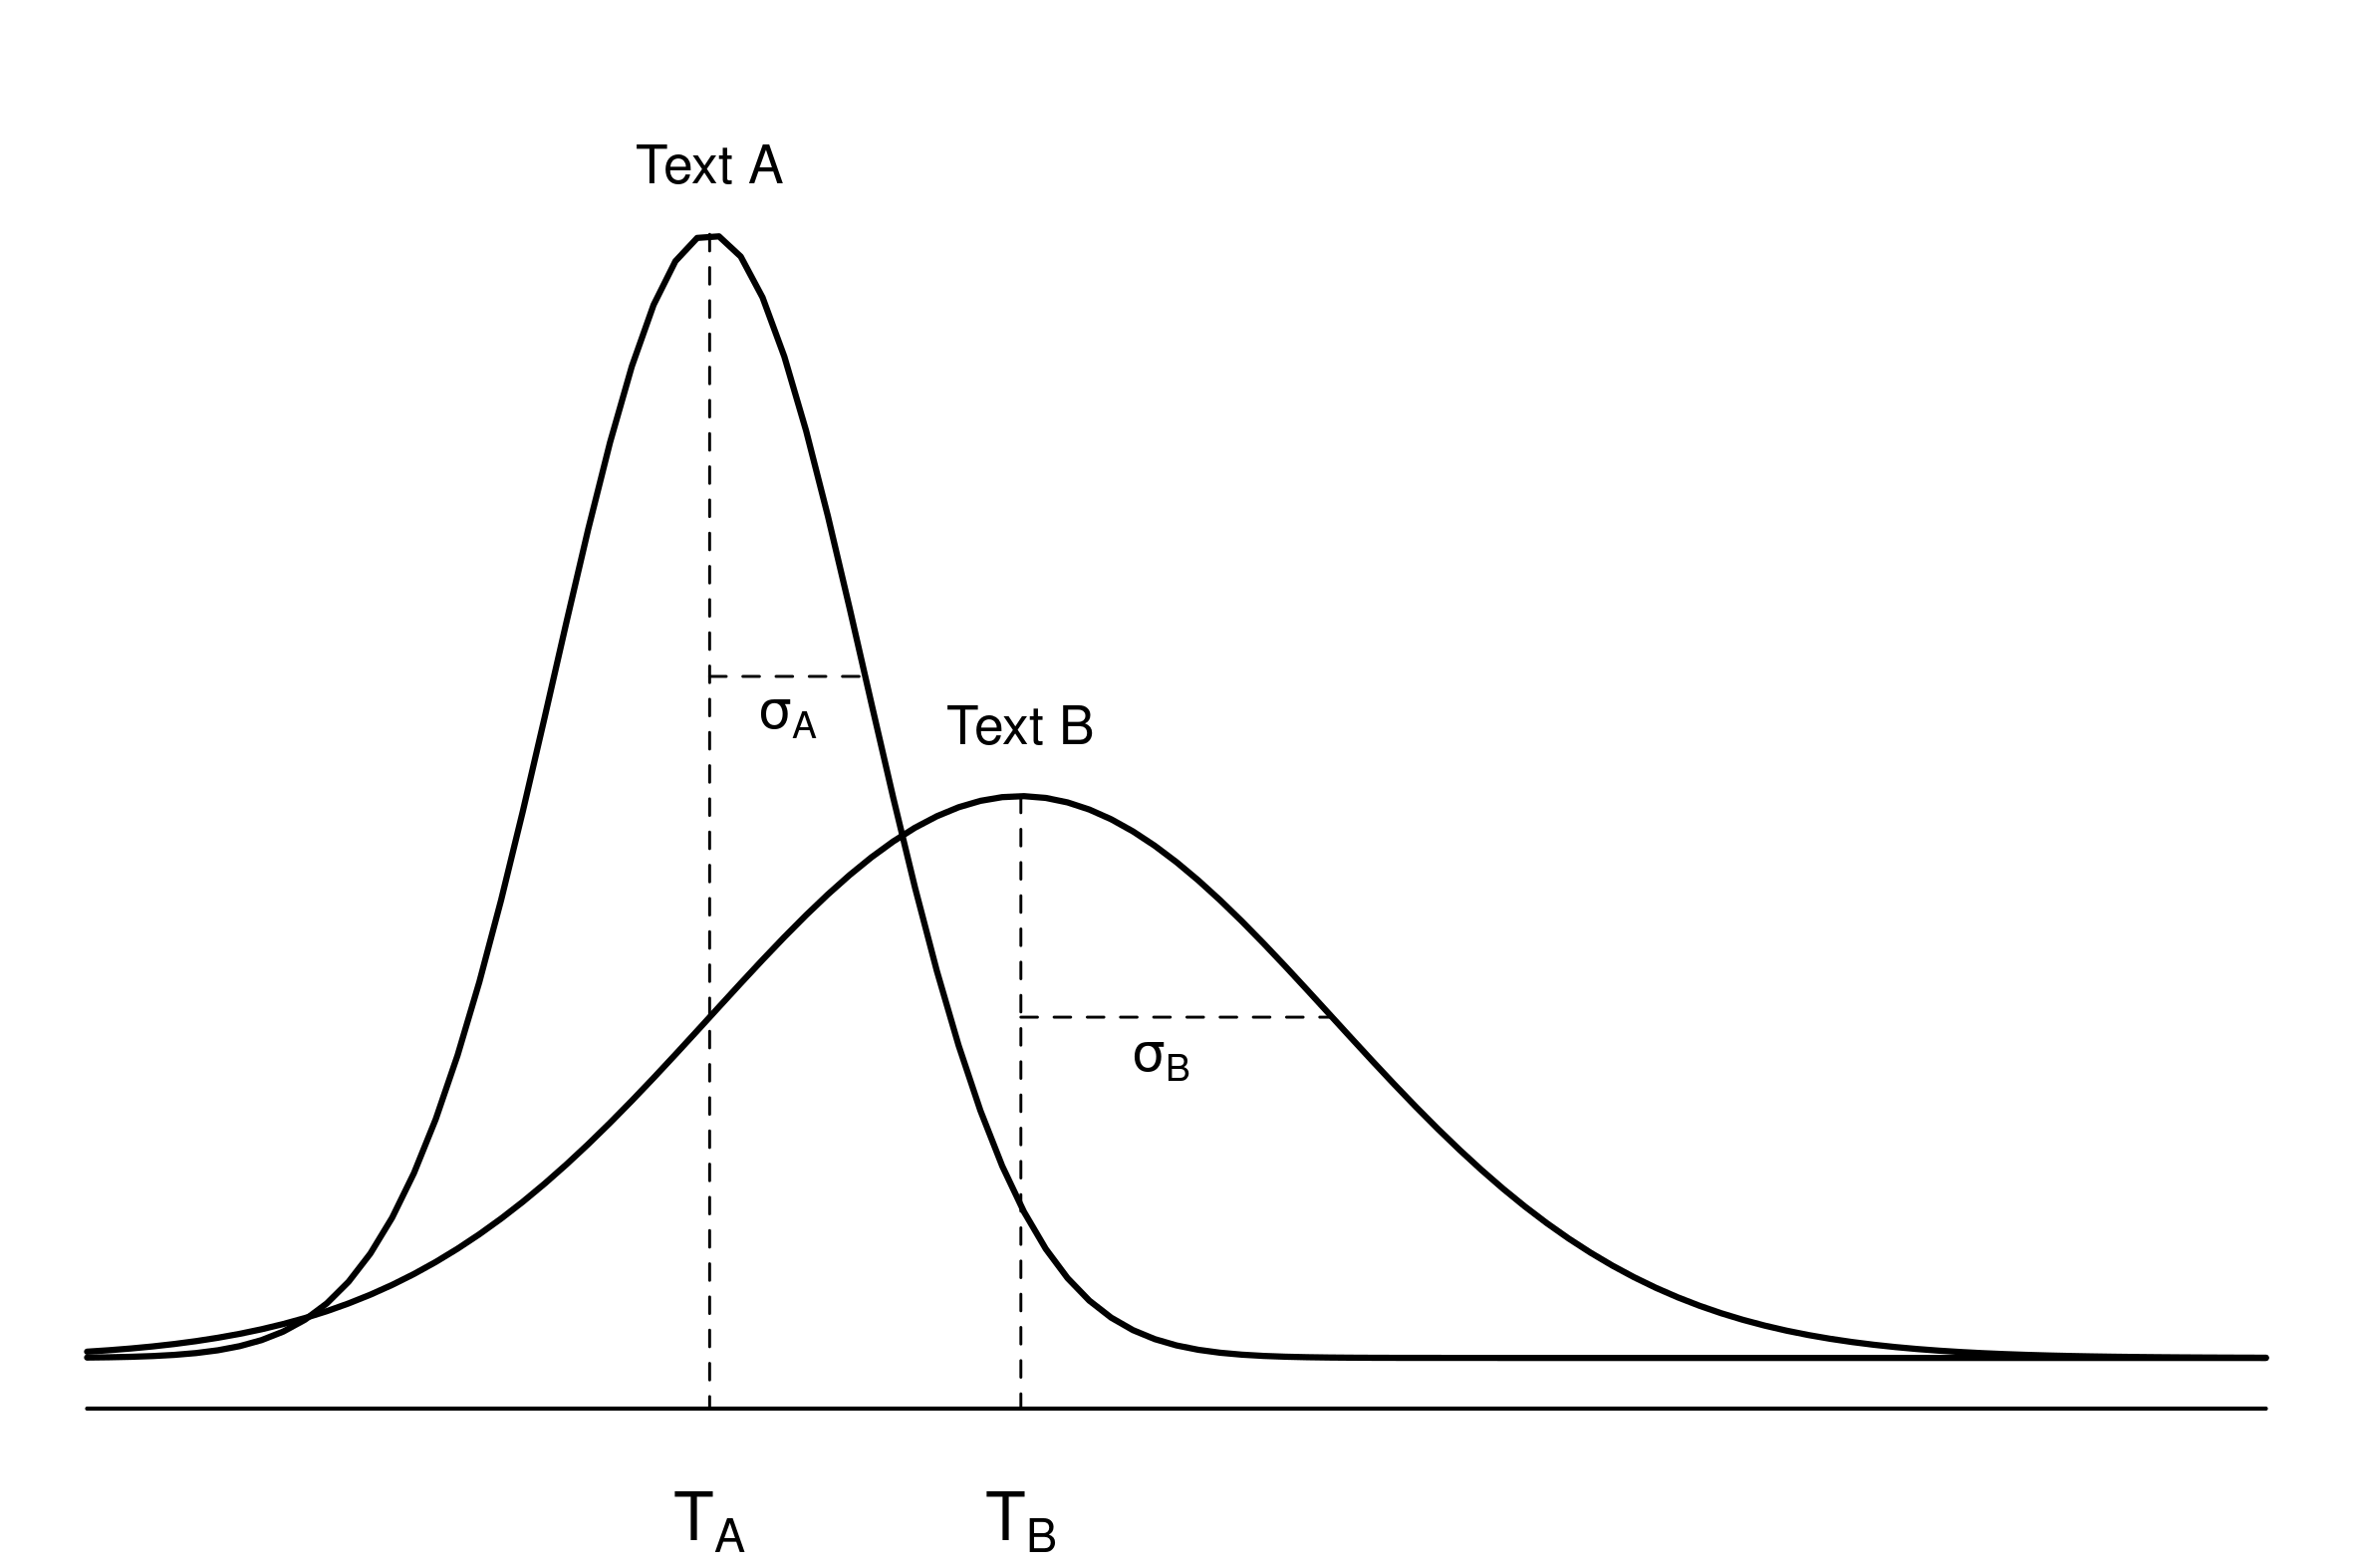
\includegraphics[width=0.7\linewidth,height=\textheight,keepaspectratio]{./images/png/discriminal_process.png}

}

\caption{\label{fig-discriminal_process}Discriminal processes for two
written texts}

\end{figure}%

However, since the individual discriminal processes of the stimuli are
not directly observable, the theory introduces \emph{the law of
comparative judgment}. This law posits that in pairwise comparisons, a
judge perceives the stimulus with a discriminal process positioned
further along the trait continuum as possessing more of the trait
\citep[pp.~251]{Bramley_2008}. This suggests that the relative distance
between stimuli, rather than their absolute positions on the continuum,
likely defines the outcome of pairwise comparisons. Indeed, the theory
assumes that the difference between the underlying discriminal processes
of the stimuli, referred to as \emph{the discriminal difference},
determines the observed dichotomous outcome. Moreover, the theory
assumes that because the individual discriminal processes form a Normal
distribution on the continuum, the discriminal difference will also
conform to a Normal distribution \citep{Andrich_1978}. In this
distribution, the mode (mean) represents the relative separation between
the stimuli, and its dispersion indicates the variability of that
separation.

Figure~\ref{fig-discriminal_difference} illustrates the distribution of
the discriminal difference for the hypothetical texts depicted in
Figure~\ref{fig-discriminal_process}. The figure indicates that the
judge perceives Text B as having significantly higher quality than Text
A. This conclusion rests on two key observations: the positive
difference between their modal discriminal processes
\((S_{B} - S_{A} > 0)\) and the probability area where the discriminal
difference distinctly favors Text B over Text A, represented by the
shaded gray area denoted as \(P(B > A)\). As a result, the dichotomous
outcome of this comparison is more likely to favor Text B over Text A.

\begin{figure}

\centering{

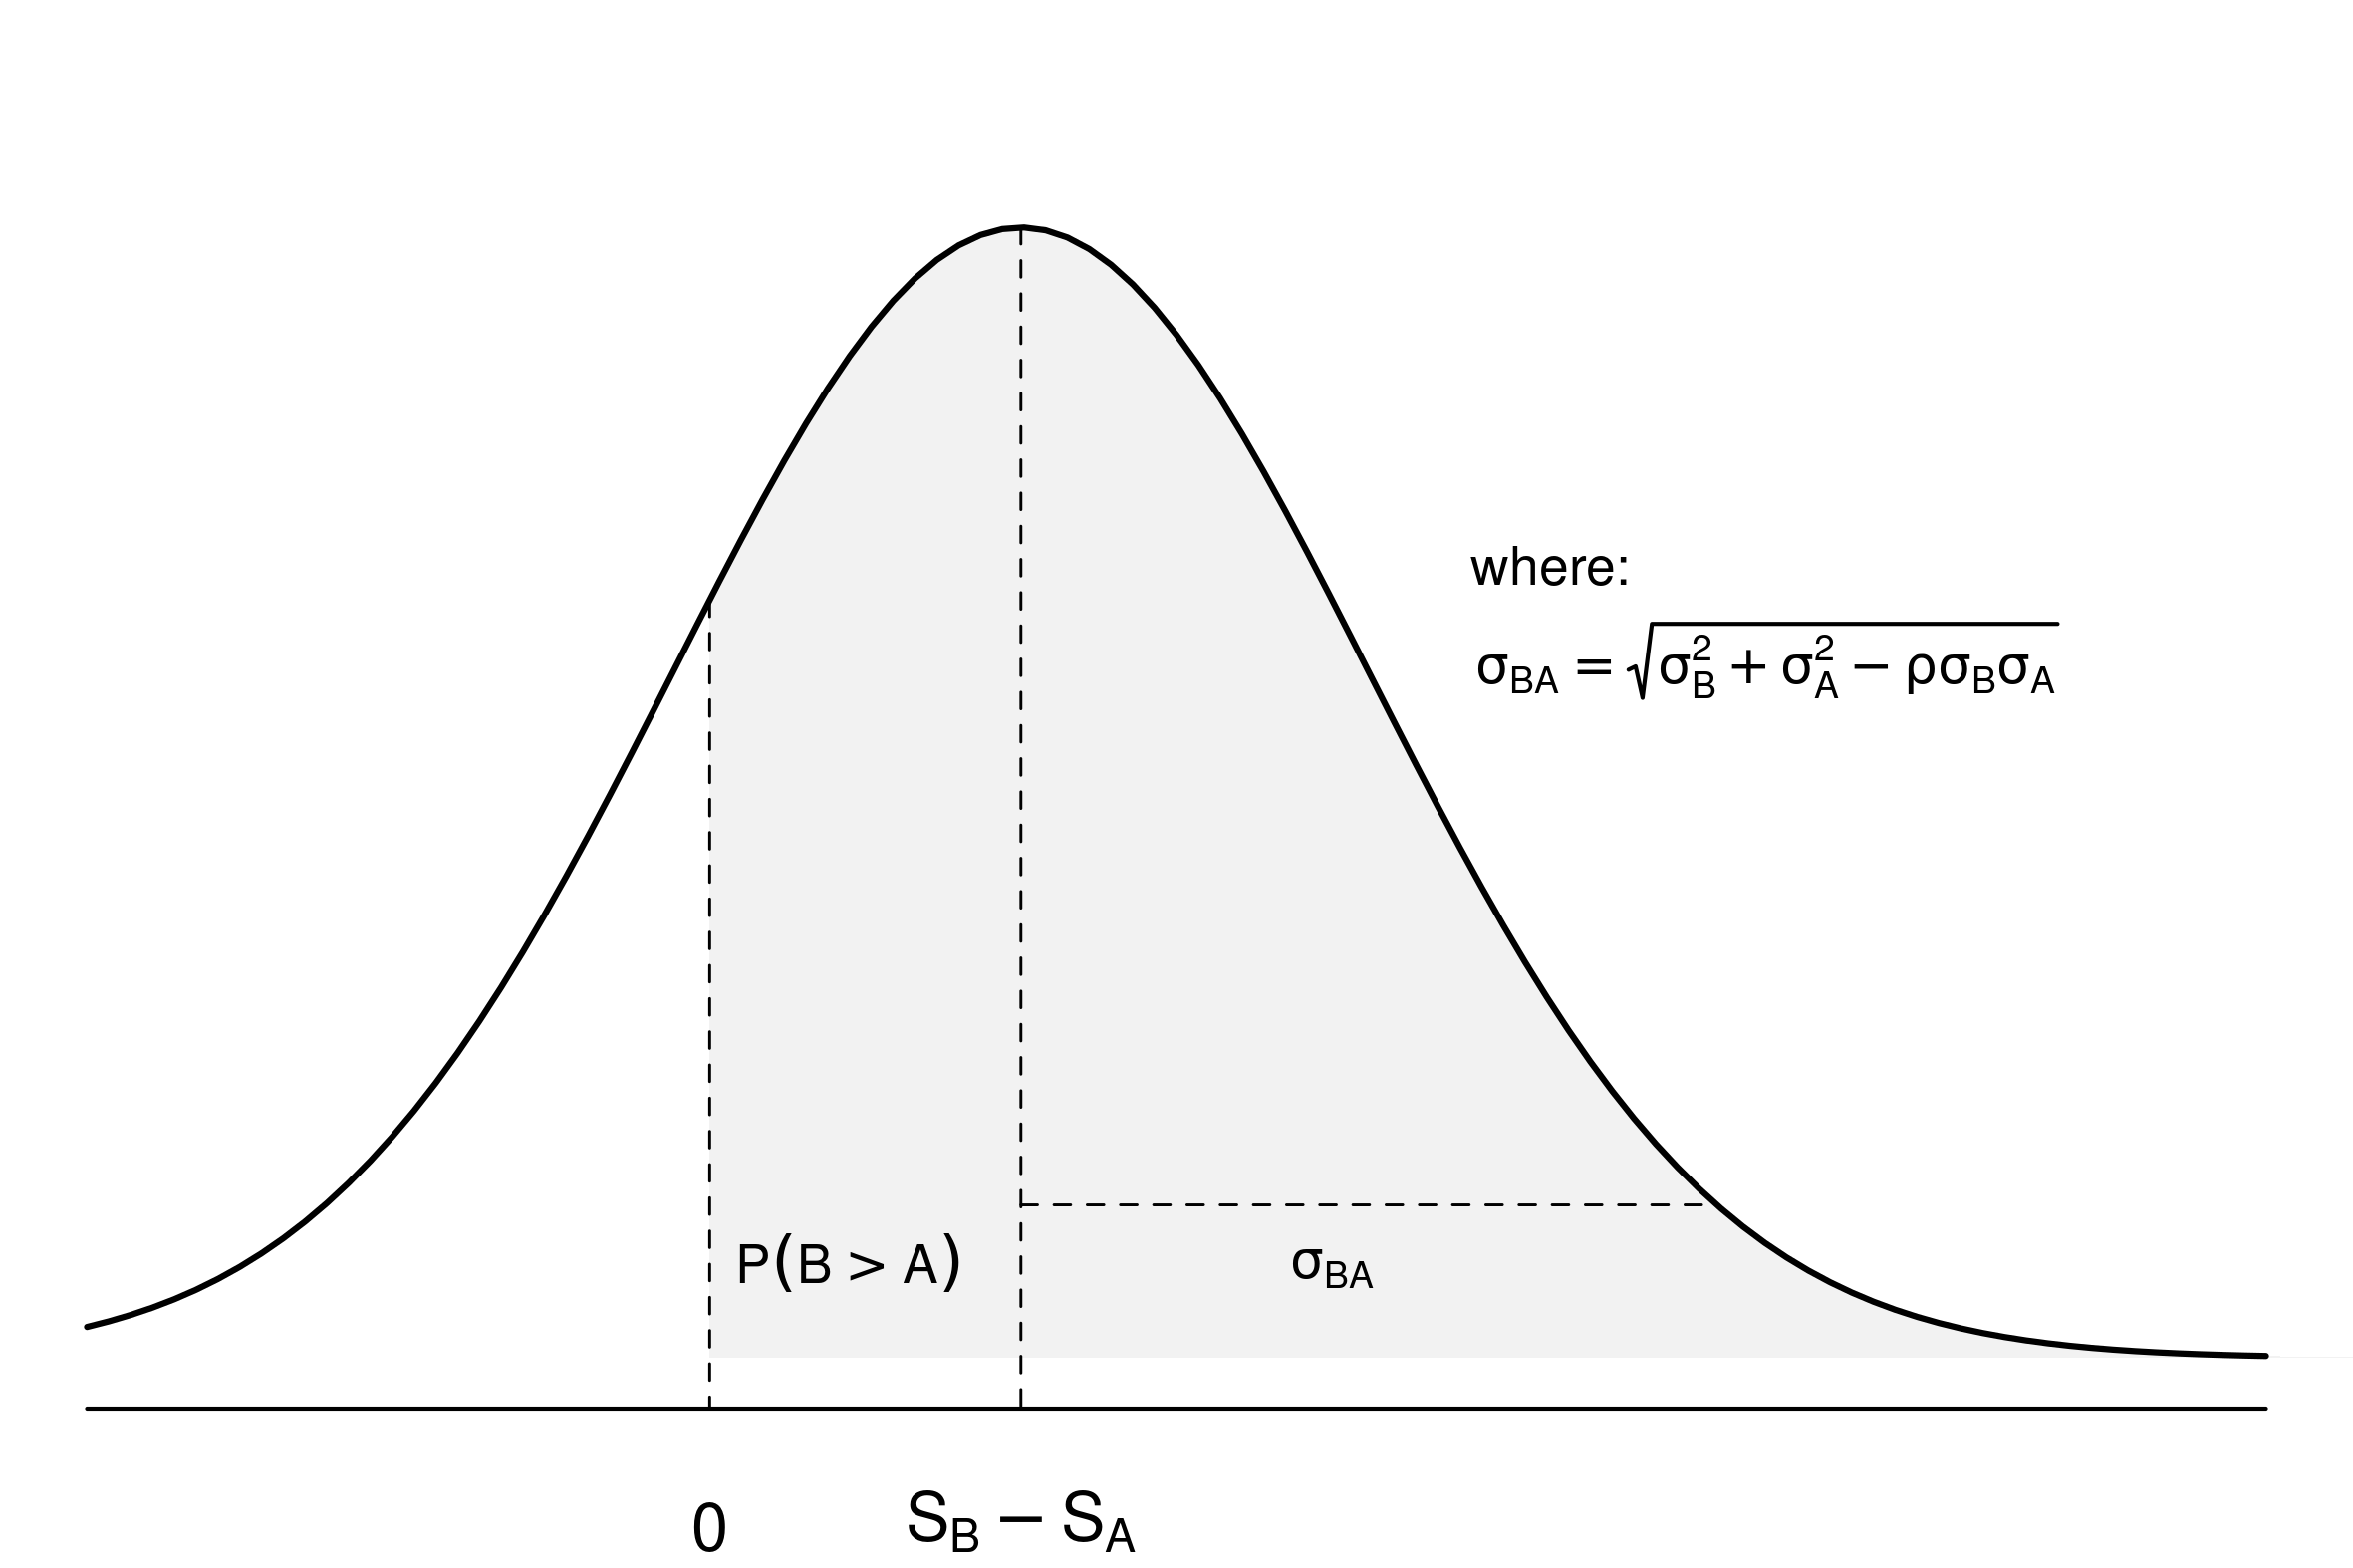
\includegraphics[width=0.7\linewidth,height=\textheight,keepaspectratio]{./images/png/discriminal_difference.png}

}

\caption{\label{fig-discriminal_difference}Discriminal difference for
two written texts}

\end{figure}%

\section{The two critical issues in CJ
literature}\label{sec-theory-issues}

This section examines the two critical issues in the CJ literature that
serve as the primary focus of this study. The first is the overreliance
on Thurstone's Case V assumptions in the statistical analysis of CJ
data. The second is the apparent disconnect between CJ's approach to
trait measurement and hypothesis testing.

\subsection{The Case V and the statistical analysis of CJ
data}\label{sec-theory-issue1}

Thurstone observed that the general form of the theory, outlined in
Section~\ref{sec-thurstone_theory}, created a trait scaling problem. The
model required estimating more ``unknown'' parameters than the available
pairwise comparisons \citep[pp.~267]{Thurstone_1927b}. To address this
issue and facilitate the practical application of the theory, he
developed five cases derived from this general form. Each case
progressively incorporated additional simplifying assumptions into the
model.

In Case I, Thurstone assumed that pairs of stimuli maintained a constant
correlation across all comparisons. In Case II, he allowed multiple
judges to make comparisons instead of restricting evaluations to a
single judge. In Case III, he introduced the assumption of zero
correlation between stimuli. In Case IV, he assumed stimuli exhibited
similar dispersions. Finally, in Case V, he replaced this assumption
with the condition that stimuli had equal discriminal dispersions.
Table~\ref{tbl-thurstone_cases} summarizes the assumptions of the
general form and the five cases. For an in-depth discussion of these
cases and their progression, refer to \citet{Thurstone_1927b} and
\citet[pp.~248--253]{Bramley_2008}.

\begin{table}

\caption{\label{tbl-thurstone_cases}Thurstones cases and their
asumptions}

\centering{

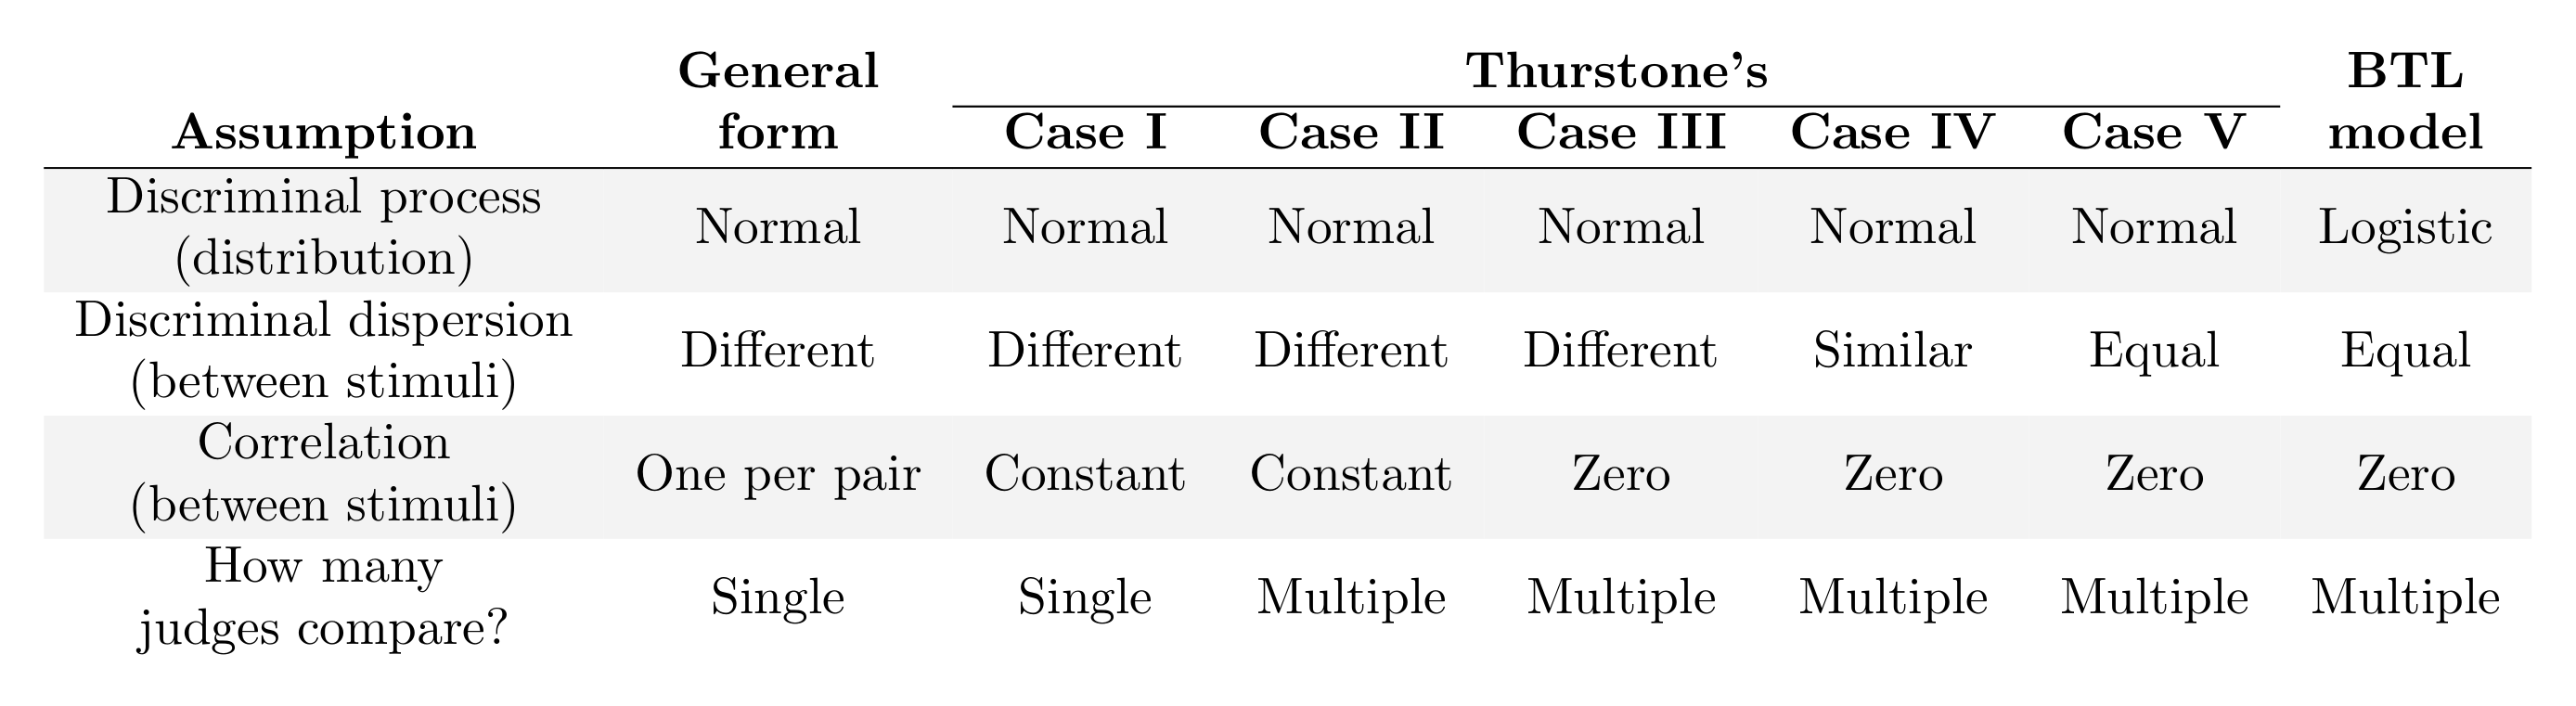
\includegraphics[width=1\linewidth,height=\textheight,keepaspectratio]{./images/png/thurstone_cases.png}

}

\end{table}%

Despite relying on the most extensive set of simplifying assumptions
\citetext{\citealp[pp.~253]{Bramley_2008}; \citealp[pp.~677]{Kelly_et_al_2022}},
Case V remains the most widely used case in the CJ literature. This
popularity stems mainly from its simplified statistical representation
in the Bradley-Terry-Luce (BTL) model
\citep{Bradley_et_al_1952, Luce_1959}. The BTL model mirrors the
assumptions of Case V, with one key difference: while Case V assumes a
Normal distribution for the stimuli's discriminal processes, the BTL
model uses the more mathematically tractable Logistic distribution
\citep[pp.~254]{Andrich_1978, Bramley_2008} (see
Table~\ref{tbl-thurstone_cases}). This substitution has little impact on
the model's estimation or interpretation, as the Normal and Logistic
distributions share similar statistical properties, differing only by a
scaling factor of approximately \(1.7\)
\citep[pp.~16]{vanderLinden_et_al_2017_I}.

However, Thurstone originally developed Case V to provide a ``rather
coarse scaling'' of traits \citep[pp.~269]{Thurstone_1927b},
prioritizing statistical simplicity over precision in trait measurement
\citep[pp.~677]{Kelly_et_al_2022}. He explicitly warned against its
untested application, stating that its use ``should not be made without
(an) experimental test'' \citep[pp.~270]{Thurstone_1927b}, acknowledging
that some assumptions could prove problematic when researchers asesss
complex traits or heterogeneous stimuli
\citep[pp.~376]{Thurstone_1927a}. Consequently, given that modern CJ
applications frequently involve such traits and stimuli, two main
assumptions of Case V and, by extension, of the BTL model may not
consistently hold in theory or practice: the assumption of equal
dispersion and zero correlation between stimuli.

\subsubsection{The assumption of equal dispersions between
stimuli}\label{sec-theory-issue1a}

According to the theory, the discriminal dispersions of stimuli play a
critical role in determining the outcome of pairwise comparisons.
Specifically, discrepancies in these dispersions shape the distribution
of the discriminal difference, directly influencing the comparison
outcome. Figure~\ref{fig-dispersion} illustrates this idea, assuming a
researcher can observe the discriminal processes for the texts shown in
Figure~\ref{fig-discriminal_process}. The figure also considers that the
discriminal dispersion for Text A remains constant and that the texts
have no correlation \((\rho=0)\).

Figure~\ref{fig-dispersion} reveals that more uncertainty in the trait
perception of Text B compared to Text A, \((\sigma_{B}-\sigma_{A})\),
broadens the distribution of their discriminal difference. This
broadening affects the probability area where the discriminal difference
distinctly favors Text B over Text A, expressed as \(P(B > A)\),
ultimately influencing the comparison outcome. Additionally, the figure
reveals that when the discriminal dispersions of the texts are equal
\((\sigma_{B}-\sigma_{A}=0)\), the discriminal difference is more likely
to favor Text B over Text A (shaded gray area), compared to situations
where their dispersions differ.

\begin{figure}

\centering{

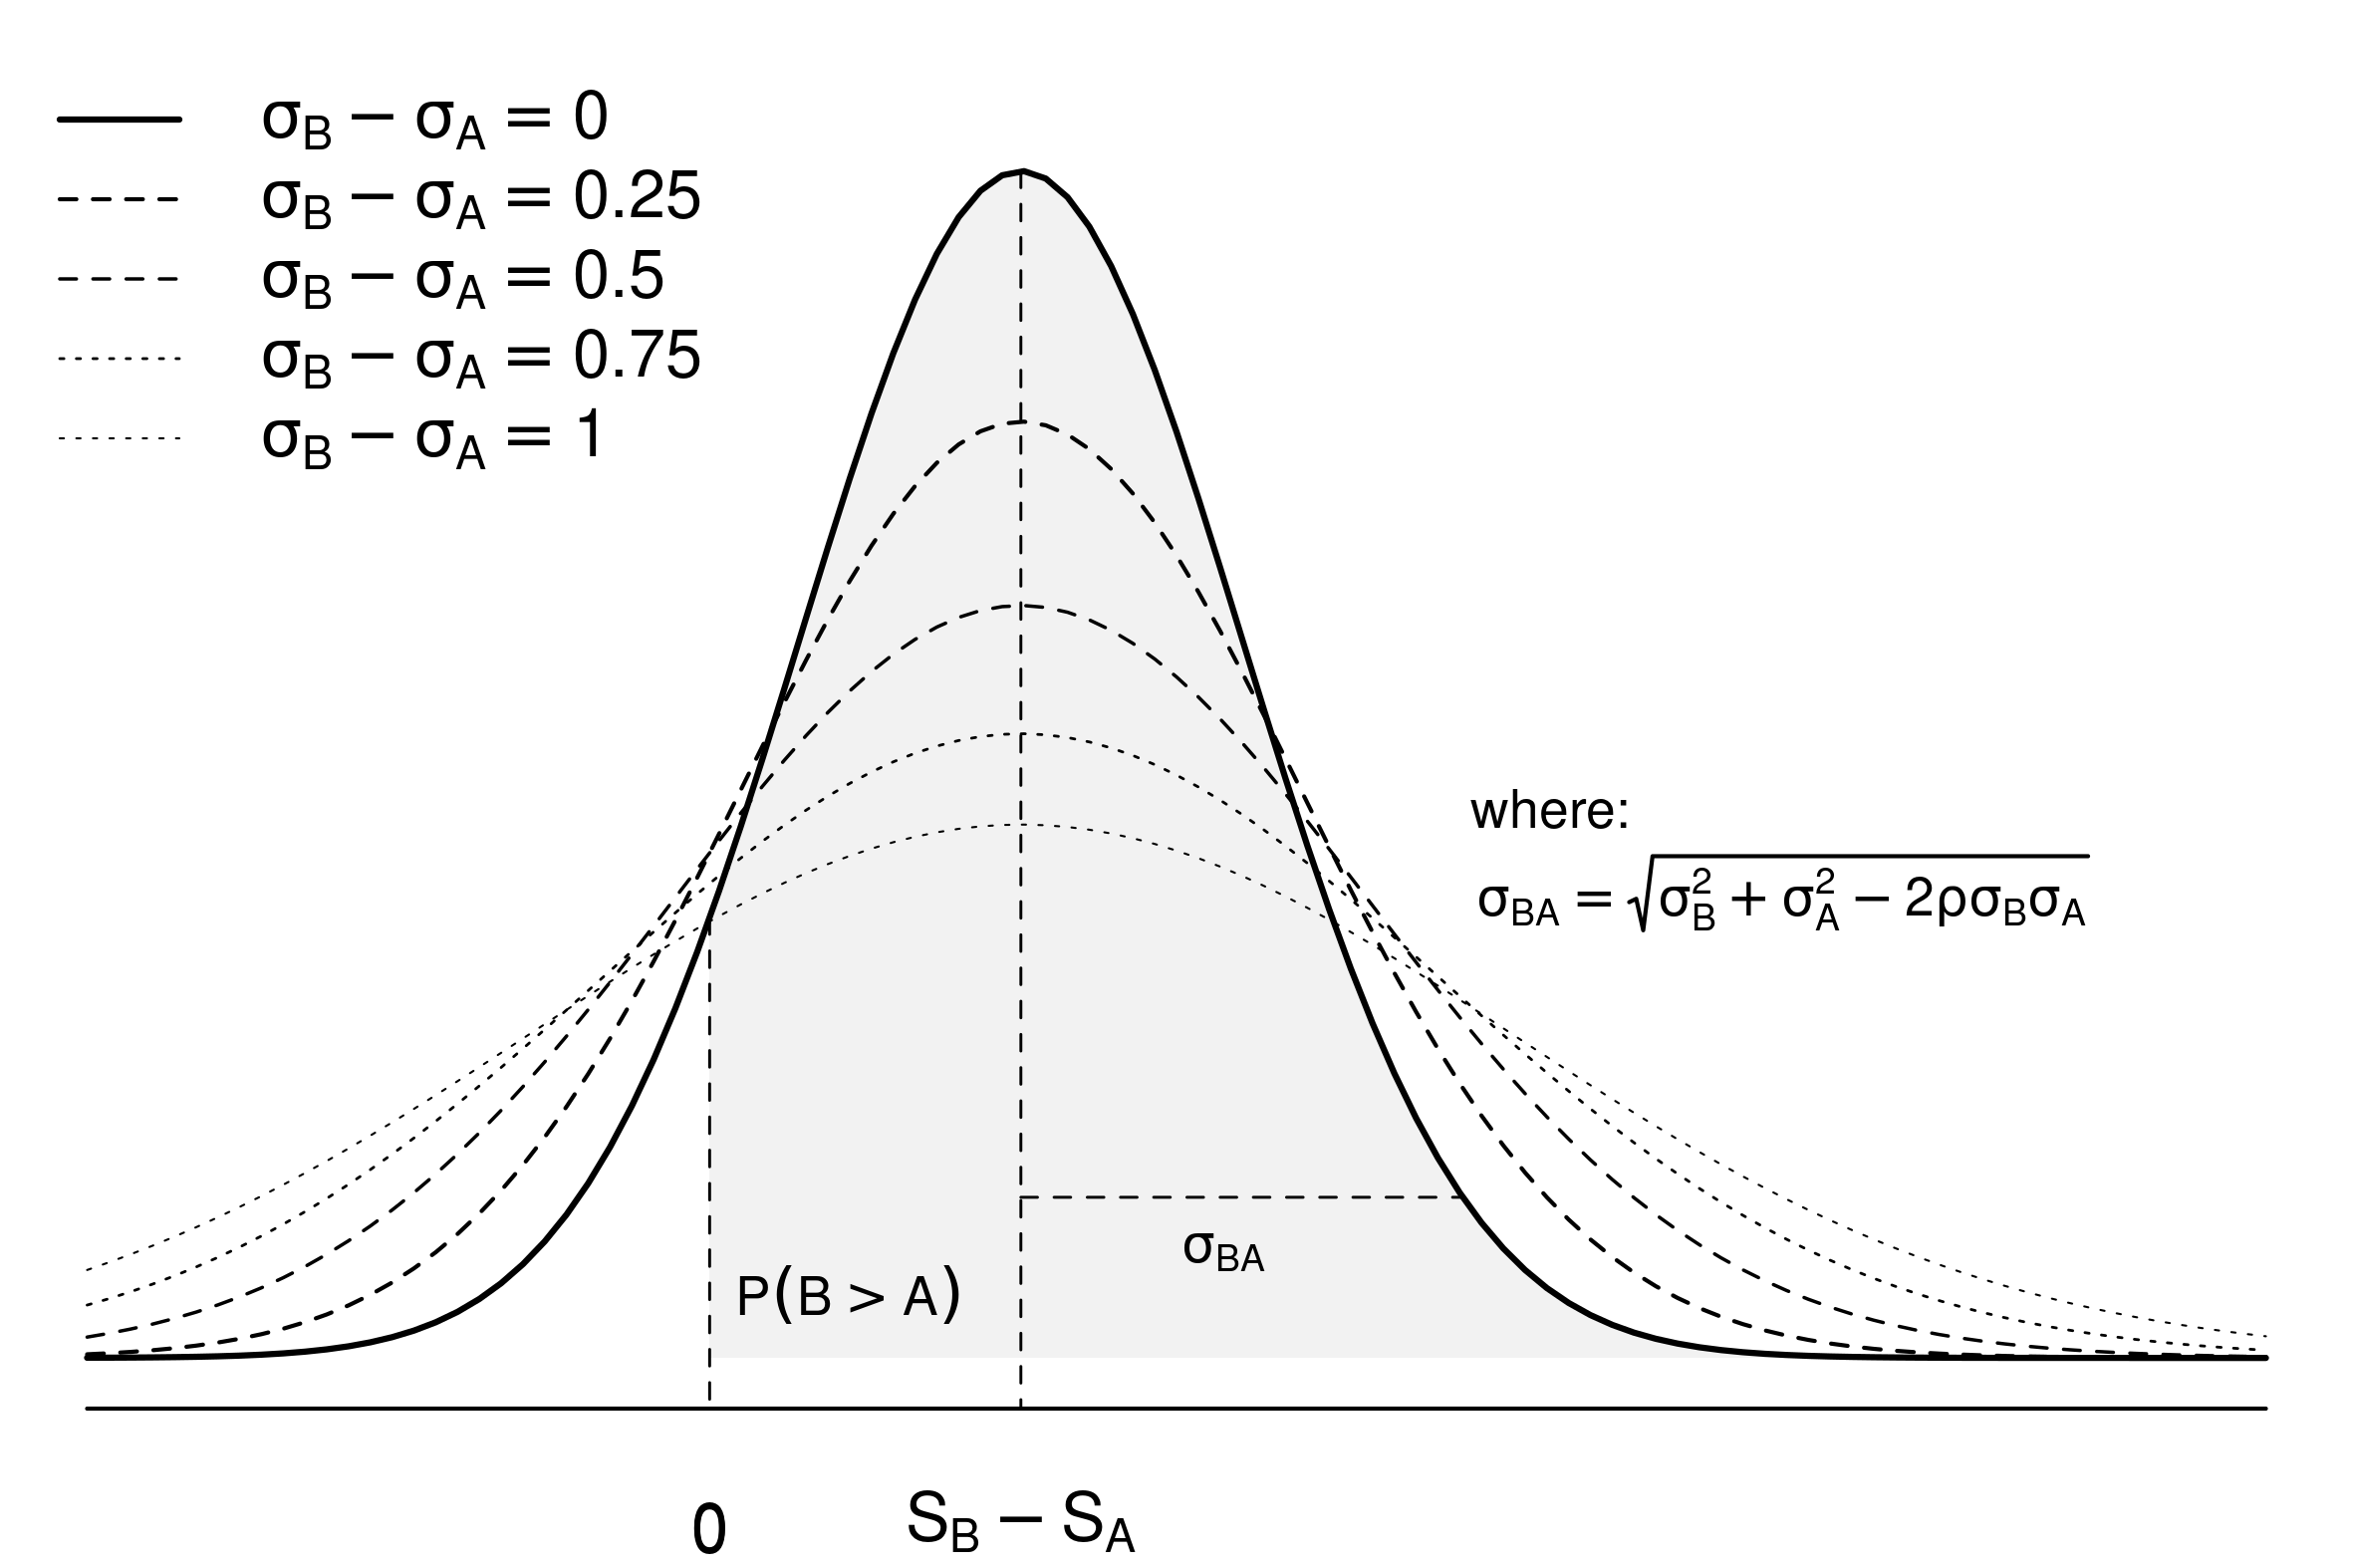
\includegraphics[width=0.7\linewidth,height=\textheight,keepaspectratio]{./images/png/dispersion.png}

}

\caption{\label{fig-dispersion}The discrepancy in the dispersions of
stimuli and their effect on the distribution of the discriminal
difference}

\end{figure}%

In experimental practice, however, this process occurs in reverse.
Researchers first observe the comparison outcome and then use the BTL
model to infer the discriminal difference between the stimuli and their
discriminal processes \citep[pp.~373]{Thurstone_1927a}. For example,
when researchers observe a large sample of outcomes favoring Text B over
Text A and correctly assume equal dispersions between the texts, the BTL
model estimates a discriminal difference distribution that accurately
represents the ``true'' discriminal difference of the texts. This
scenario is illustrated with Figure~\ref{fig-dispersion} when the
discriminal difference distribution of the model aligns with the
``true'' distribution, represented by the thick continuous line
corresponding to \(\sigma_{B}-\sigma_{A}=0\). The estimation accuracy of
this discriminal difference, in turn, ensures reliable discriminal
process estimates for the texts (citation needed?). It then intuitively
follows that the outcome's ability to represent the ``true'' differences
between stimuli largely depends on the validity of the model's
assumptions, particularly the assumption of equal dispersions.

However, Thurstone contended that the assumption of equal dispersions
may not hold when researchers assess complex traits or heterogeneous
stimuli \citep[pp.~376]{Thurstone_1927a}, as these traits and stimuli
can introduce judgment discrepancies due to their unique features
\citep{vanDaal_et_al_2016, Lesterhuis_2018, Chambers_et_al_2022}.
Indeed, evidence of this violation may already exist in the CJ
literature as misfit statistics, which measure judgment discrepancies
associated with specific stimuli
\citetext{\citealp[pp.~12]{Pollitt_2004}; \citealp[pp.~20]{Goossens_et_al_2018}}.
For example, labeling texts as ``misfits'' indicates that comparisons
involving these texts result in more judgment discrepancies than those
involving other texts
\citep{Pollitt_2012a, Pollitt_2012b, vanDaal_et_al_2016, Goossens_et_al_2018}.
These discrepancies, in turn, suggest that the discriminal differences
for ``misfit'' texts have broader distributions, indicating that their
discriminal processes may also exhibit more variation than that of other
texts. A similar reasoning applies to ``misfit'' judges, whose
evaluations deviate substantially from the shared consensus due to the
unique characteristics of the stimuli or the judges themselves.
Moreover, these ``misfit'' judges and their deviations can introduce
additional statistical and measurement issues, which we discuss in
Section~\ref{sec-theory-issue1b}.

Then, incorrectly assuming equal dispersions between stimuli can lead
the BTL model to introduce various statistical and measurement issues.
For example, the model could overestimate the accuracy of the outcome in
reflecting the ``true'' discriminal differences between stimuli. This
overestimation may result in spurious inferences about these differences
\citep[pp.~370]{McElreath_2020} and, by extension, about the stimuli's
discriminal processes. Figure~\ref{fig-dispersion} also illustrates this
scenario when the model's discriminal difference distribution aligns
with the thick continuous line for \(\sigma_{B}-\sigma_{A}=0\), while
the ``true'' discriminal difference follows any discontinuous line where
\(\sigma_{B}-\sigma_{A} \neq 0\). Moreover, if researchers recognize
that misfit statistics highlight critical differences in dispersions,
the common practice in CJ literature of excluding stimuli based on these
statistics
\citep{Pollitt_2012a, Pollitt_2012b, vanDaal_et_al_2016, Goossens_et_al_2018}
may inadvertently discard valuable information, introducing bias into
trait estimates \citep[chap.~12]{Zimmerman_1994, McElreath_2020}. These
biases are often unpredictable, as they depend on the specific stimuli
excluded from the analysis.

\subsubsection{The assumption of zero correlation between
stimuli}\label{sec-theory-issue1b}

Denoted by \(\rho\), the correlation measures the dependence of a
judge's perception of the trait in one stimulus on his perception of the
same trait in another. Like the discriminal dispersions, this
correlation shapes the distribution of the discriminal difference and
directly influences the outcomes of pairwise comparisons.
Figure~\ref{fig-correlation} illustrates this concept, assuming the
researcher can observe the discriminal processes for the texts shown in
Figure~\ref{fig-discriminal_process}. The figure also considers that the
discriminal dispersions for both texts remain constant.

Figure~\ref{fig-correlation} reveals that as the correlation between the
texts increases, the distribution of their discriminal difference
becomes narrower. This narrowing affects the area under the curve where
the discriminal difference distinctly favors Text B over Text A, denoted
as \(P(B > A)\), thus influencing the comparison outcome. Furthermore,
the figure shows that when two texts are independent or uncorrelated
\((\rho=0)\), their discriminal difference is less likely to favor Text
B over Text A (shaded gray area), compared to scenarios when the texts
are highly correlated.

\begin{figure}

\centering{

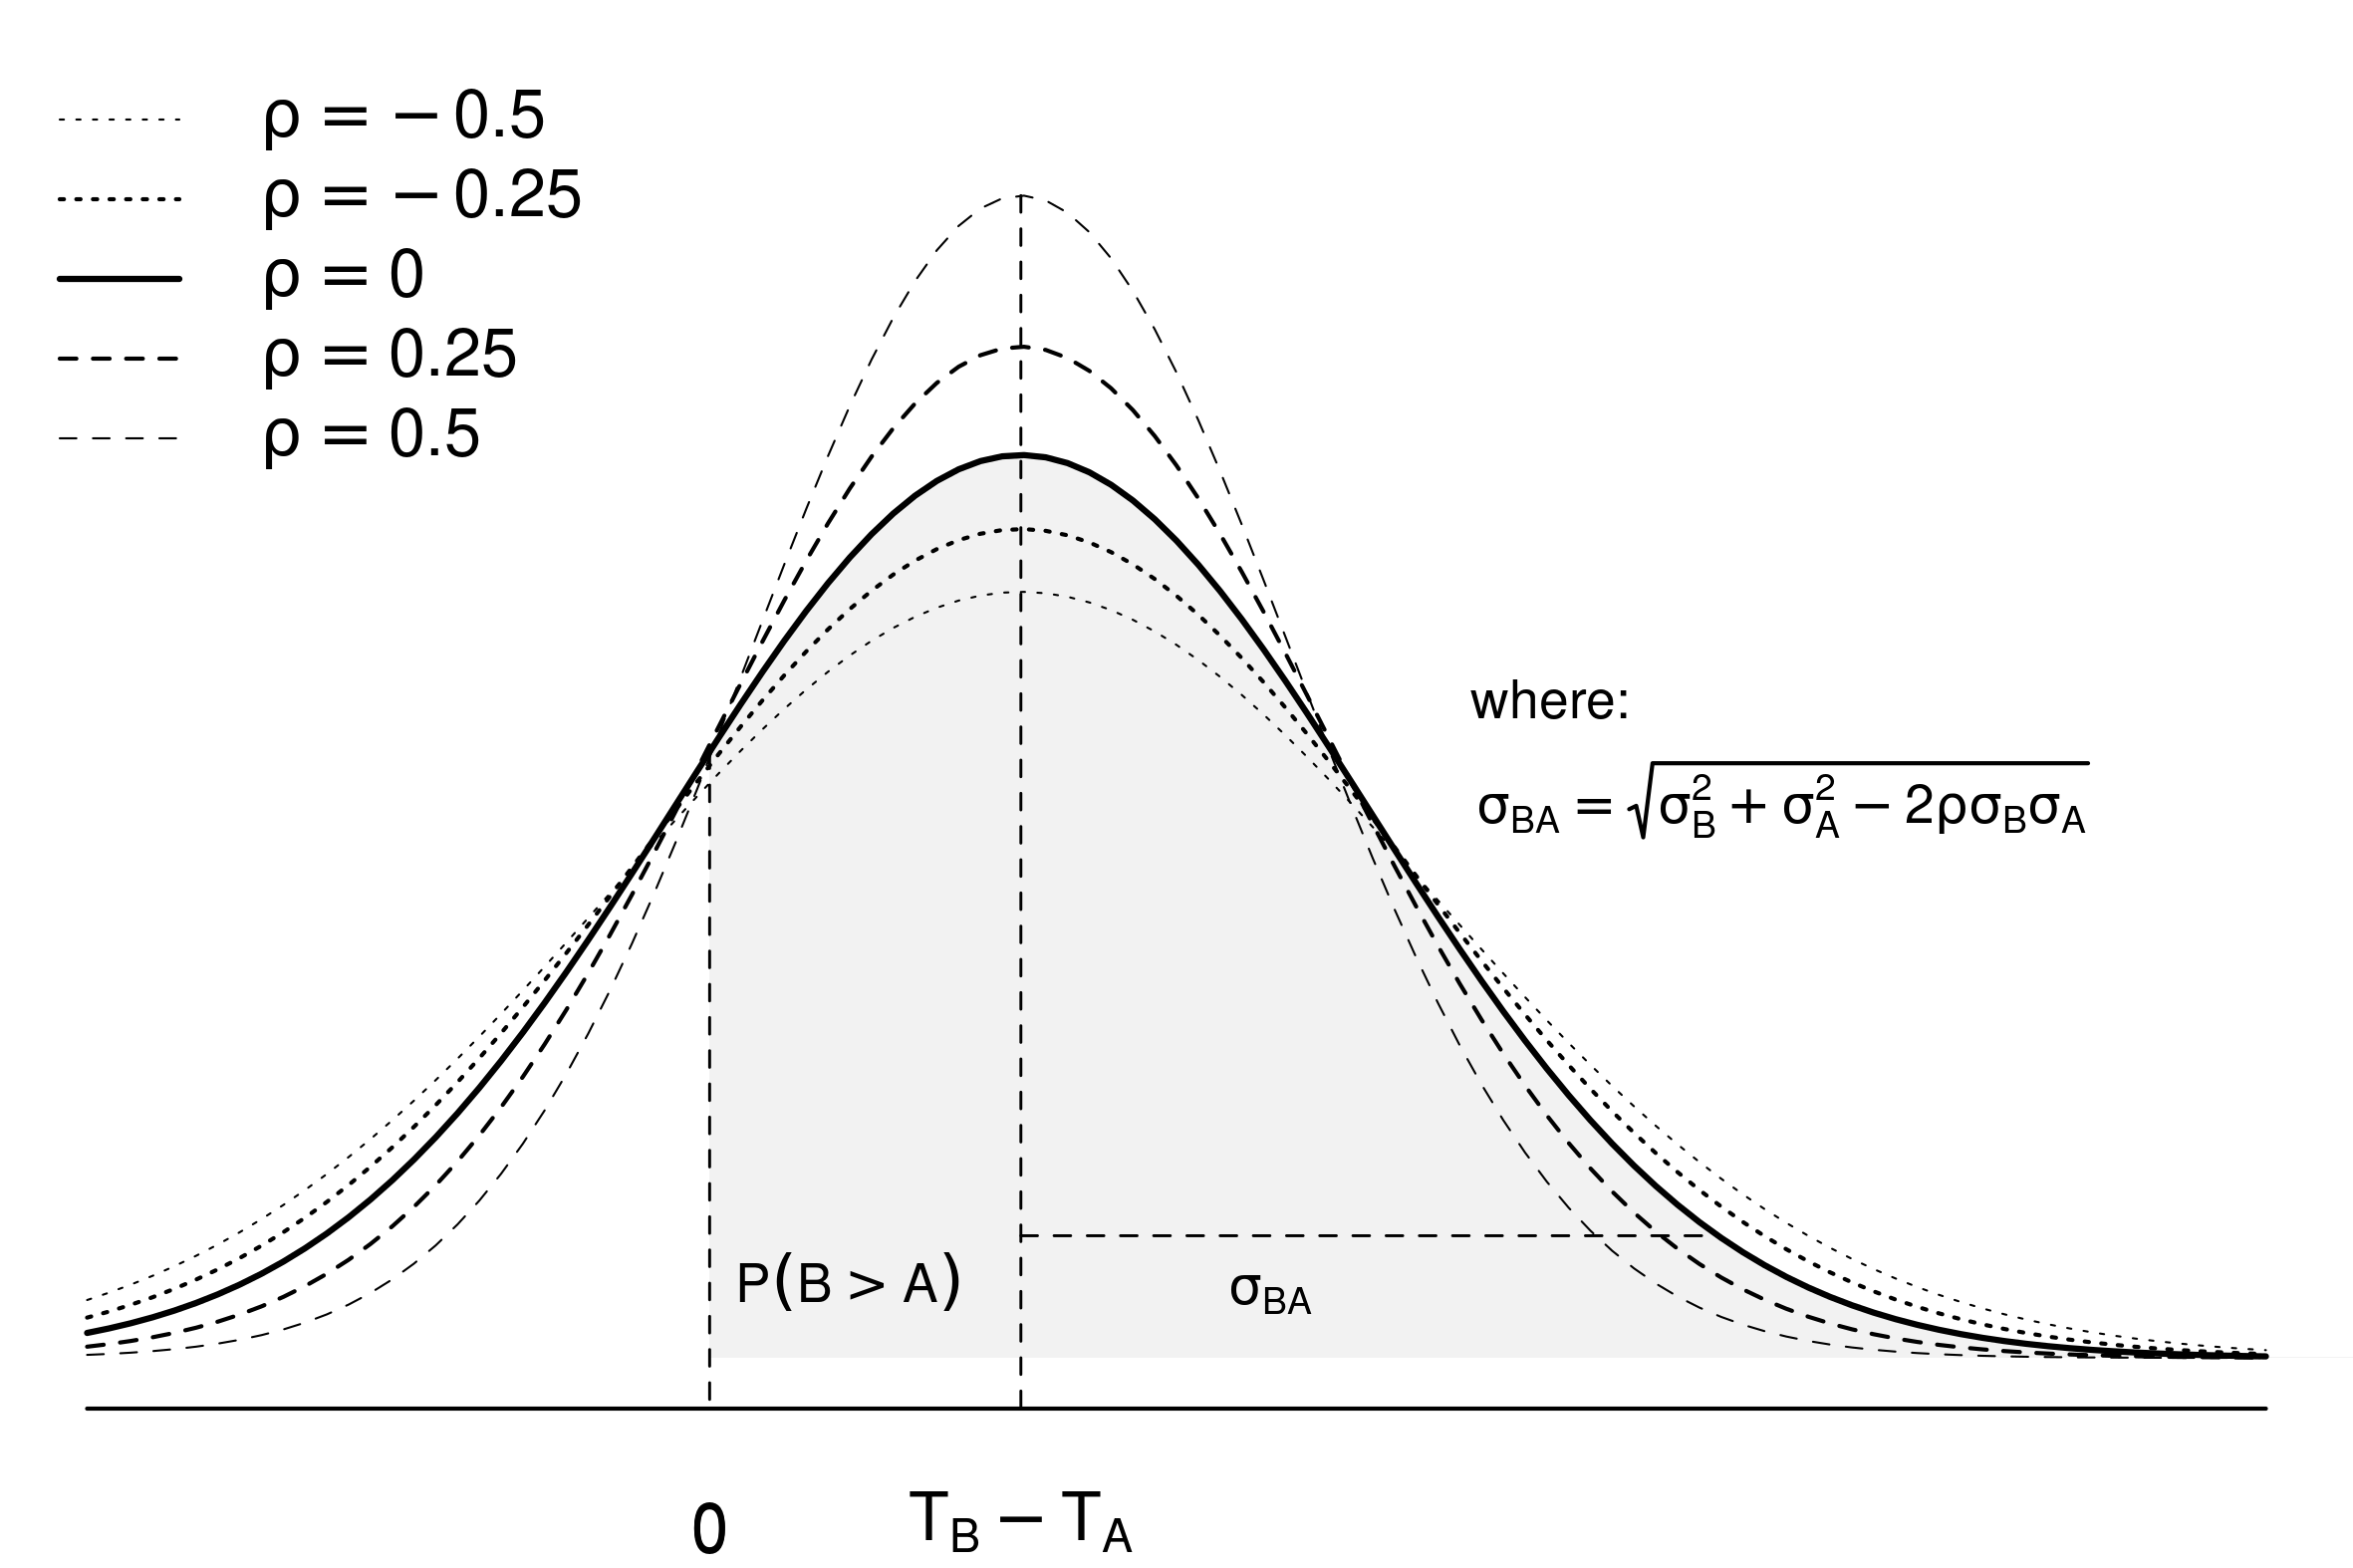
\includegraphics[width=0.7\linewidth,height=\textheight,keepaspectratio]{./images/png/correlation.png}

}

\caption{\label{fig-correlation}The correlation between stimuli and its
effect on the distribution of the discriminal difference}

\end{figure}%

However, in experimental practice, researchers typically follow this
process in reverse. For example, when they observe a large sample of
outcomes favoring Text B over Text A and correctly assume zero
correlation between the texts, the BTL model estimates a discriminal
difference distribution that accurately represents the ``true''
discriminal difference of the texts. This scenario is illustrated with
Figure~\ref{fig-correlation} when the discriminal difference
distribution of the model aligns with the ``true'' distribution,
represented by the thick continuous line corresponding to \(\rho=0\).
The accuracy of this discriminal difference estimation, in turn, ensures
reliable estimates for the discriminal process of the texts (citation
needed?).

Notably, Thurstone's Case V and the BTL model assume independent
discriminal processes across comparisons. Thurstone attributed this
independence to the cancellation of potential judges' biases, driven by
two opposing and equally weighted effects occurring during the pairwise
comparisons \citep[pp.~268]{Thurstone_1927b}. \citet{Andrich_1978}
mathematically demonstrated this cancellation using the BTL model under
the assumption of discriminal processes with additive biases. However,
it is easy to imagine at least two scenarios where the zero correlation
assumption almost certainly does not hold: when the pairwise comparison
involves multidimensional, complex traits with heterogeneous stimuli and
when an additional hierarchical structure is relevant to the stimuli.

In the first scenario, the intricate aspects of multidimensional,
complex traits may introduce dependencies between the stimuli due to
certain judges' biases that resist cancellation. Research on text
quality suggests that when judges evaluate these traits, they often rely
on various intricate characteristics of the stimuli to form their
judgments
\citep{vanDaal_et_al_2016, Lesterhuis_2018, Chambers_et_al_2022}. These
additional relevant characteristics, which are unlikely to be equally
weighted or opposing, can unevenly influence judges' perceptions,
creating biases in their judgments and, ultimately, introducing
dependencies between stimuli
\citep[pp.~346]{vanderLinden_et_al_2017_II}. For example, this could
occur when a judge assessing the argumentative quality of a text places
more weight on its grammatical accuracy than other judges, ultimately
favoring texts with fewer errors but weaker arguments. While direct
evidence for this specific scenario is lacking, studies such as
\citet{Pollitt_et_al_2003} demonstrate the presence of such biases,
supporting the idea that the factors influencing pairwise comparisons
may not always cancel out.

In the second scenario, the shared context or inherent connections
created by additional hierarchical structures may further introduce
dependencies between stimuli, a statistical phenomenon commonly known as
clustering \citep{Everitt_et_al_2010}. Although the CJ literature
acknowledges the presence of such hierarchical structures, the
statistical handling of this extra source of dependency between stimuli
has been inadequate. For example, when CJ data includes multiple samples
of stimuli from the same individuals, researchers often rely on
(average) estimated BTL scores to conduct subsequent analyses and tests
at the individual hierarchical level
\citep{Bramley_et_al_2019, Boonen_et_al_2020, Bouwer_et_al_2023, vanDaal_et_al_2017, Jones_et_al_2019, Gijsen_et_al_2021}.
However, this approach can introduce additional statistical and
measurement issues, which we discuss in Section~\ref{sec-theory-issue2}.

{In any case, similar to Section~\ref{sec-theory-issue1a}, incorrectly
assuming zero correlation between stimuli can lead the BTL model to
introduce various statistical and measurement issues. For instance, the
model could over- or underestimate the accuracy of the outcome in
reflecting the ``true'' discriminal differences between stimuli. This
over- underestimation may result in spurious inferences about these
differences and, by extension, about the stimuli's discriminal processes
\citep[pp.~341]{Hoyle_et_al_2023}. Figure~\ref{fig-correlation} also
illustrates this scenario when the model's discriminal difference
distribution aligns with the thick continuous line for \(\rho=0\), while
the ``true'' discriminal difference follows any discontinuous line where
\(\rho \neq 0\). This missaligment can be due to the overlook of
additional relevant traits, such as judges' biases, which cause
dimensional mismatches in the BTL model, artificially inflating the
reliability of the trait \citep[pp.~341]{Hoyle_et_al_2023} or, even
worse, introduce bias into the trait's estimates \citep{Ackerman_1989}.
Furthermore, researchers who exclude judges based on misfit statistics
can risk discarding valuable information, further biasing the trait's
estimates \citep[chap.~12]{Zimmerman_1994, McElreath_2020}. Lastly,
researchers who fail to account for hierarchical (grouping) structures
can reduce the precision of model parameter estimates, which may amplify
the overestimation of the trait's reliability
\citep[pp.~482]{Hoyle_et_al_2023}.}

\subsection{The disconnect between trait measurement and hypothesis
testing}\label{sec-theory-issue2}

Building on the previous section, it is clear that, despite its
limitations, the BTL model is commonly used as the measurement model in
CJ assessments. A measurement model specifies how manifest variables
contribute to the estimation of latent variables
\citep{Everitt_et_al_2010}. For example, when evaluating text quality,
researchers use the BTL model to process the dichotomous outcomes
resulting from the pairwise comparisons (the manifest variables) to
estimate scores that reflect the underlying quality level of the texts
(the latent variable)
\citep{Laming_2004, Pollitt_2012b, Whitehouse_2012, vanDaal_et_al_2016, Lesterhuis_2018_thesis, Coertjens_et_al_2017, Goossens_et_al_2018, Bouwer_et_al_2023}.

Researchers then typically use these estimated BTL scores, or their
transformations, to conduct additional analyses or hypothesis tests. For
example, these scores have been used to identify `misfit' judges and
stimuli \citep{Pollitt_2012b, vanDaal_et_al_2016, Goossens_et_al_2018},
detect biases in judges' ratings
\citep{Pollitt_et_al_2003, Pollitt_2012b}, calculate correlations with
other assessment methods \citep{Goossens_et_al_2018, Bouwer_et_al_2023},
or test hypotheses related to the underlying trait of interest
\citep{Bramley_et_al_2019, Boonen_et_al_2020, Bouwer_et_al_2023, vanDaal_et_al_2017, Jones_et_al_2019, Gijsen_et_al_2021}.

However, the statistical literature advises caution when using estimated
scores for additional analyses and tests. A key consideration is that
BTL scores are parameter estimates that inherently carry uncertainty.
Ignoring this uncertainty can bias the analysis and reduce the precision
of hypothesis tests. Notably, the direction and magnitude of such biases
are often unpredictable. Results may be attenuated, exaggerated, or
remain unaffected depending on the degree of uncertainty in the scores
and the actual effects being tested
\citetext{\citealp[pp.~25]{Kline_et_al_2023}; \citealp[pp.~137]{Hoyle_et_al_2023}}.
Finally, the reduced precision in hypothesis tests diminishes their
statistical power, increasing the likelihood of committing type-I or
type-II errors \citep{McElreath_2020}.

{In aggregate, researchers' inadequate handling of violations to the
assumptions of equal dispersion and zero correlation between stimuli,
along with the apparent disconnect between CJ's approach to trait
measurement and hypothesis testing, can undermine the reliability of the
trait estimates and ultimately compromise its validity
\citep[pp.~2]{Perron_et_al_2015}. Consequently, adopting a more
systematic and integrated approach to examining what happens when judges
compare two stimuli could offer several statistical and measurement
benefits, including addressing these issues.}

\section{An updated theoretical and statistical model for
CJ}\label{sec-theory}

This section presents a theoretical model for CJ that extends
Thurstone's theory. The model systematically incorporates all factors
involved when judges make pairwise comparisons. Additionally, the
section develops the statistical translation of the theoretical model
based on assumptions informed by the CJ theory.

\subsection{The theoretical model}\label{sec-theory-theoretical}

The (latent) discriminal difference of the stimuli directly determines
the (manifest) outcome of the pairwise comparisons

\begin{figure}

\centering{

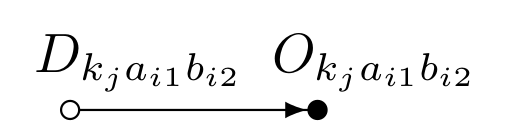
\includegraphics[width=0.29\linewidth,height=\textheight,keepaspectratio]{./images/png/CJ_TM_A1.png}

}

\caption{\label{fig-CJ_TM_A1}Theoretical model A1\$}

\end{figure}%

The (latent) ``perceived'' discriminal processes for the stimuli
directly determines their discriminal difference

\begin{figure}

\centering{

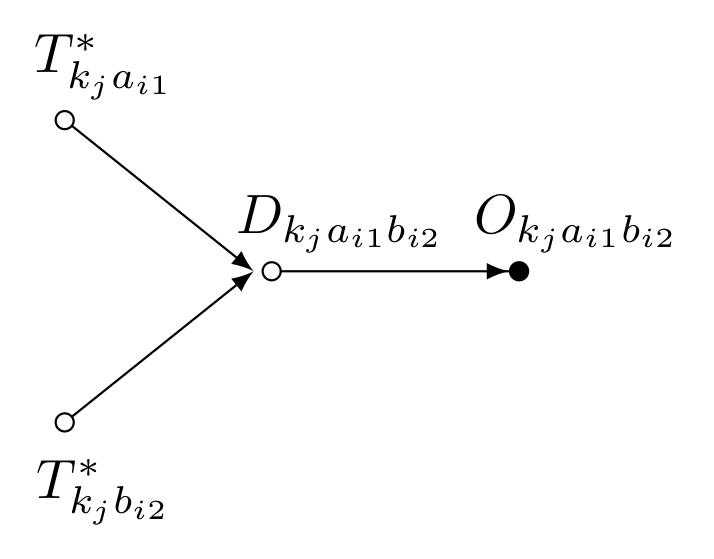
\includegraphics[width=0.4\linewidth,height=\textheight,keepaspectratio]{./images/png/CJ_TM_A2.png}

}

\caption{\label{fig-CJ_TM_A2}Theoretical model A2\$}

\end{figure}%

The (latent) ``true'' discriminal processes for the stimuli and the
judges' biases directly determines their (latent) ``perceived''
discriminal processes

\begin{figure}

\centering{

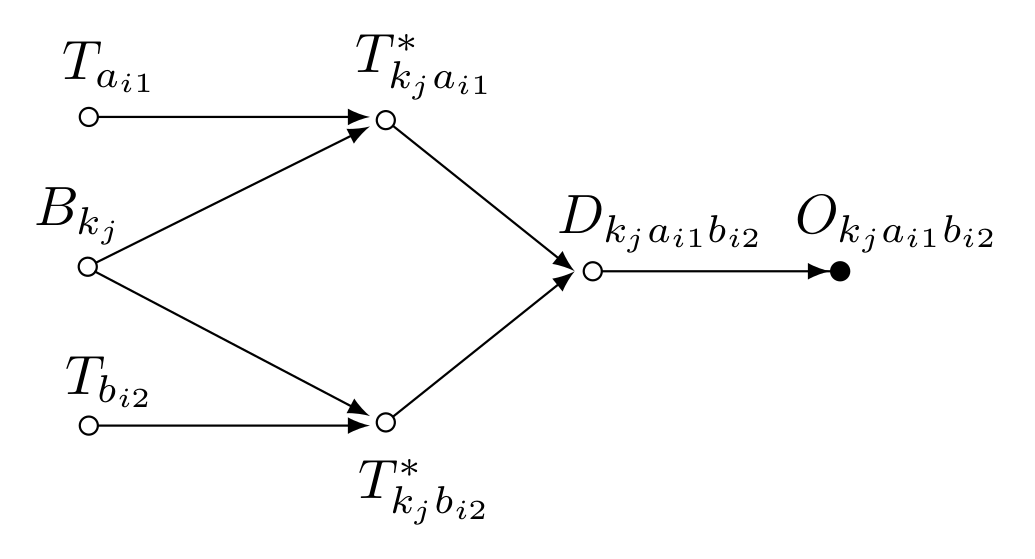
\includegraphics[width=0.6\linewidth,height=\textheight,keepaspectratio]{./images/png/CJ_TM_A3.png}

}

\caption{\label{fig-CJ_TM_A3}Theoretical model A3\$}

\end{figure}%

without loosing generality, the (latent) ``perceived'' and ``true''
discriminal processes for the stimuli can be depicted in a vector for
each judge, as in

\subsection{From theory to statistics}\label{sec-theory-statistics}

\section{Discussion}\label{sec-discuss}

\subsection{Findings}\label{sec-discuss-finding}

\subsection{Limitations and further
research}\label{sec-discuss-limitations}

\section{Conclusion}\label{sec-conclusion}

\newpage{}

\section*{Declarations}\label{declarations}
\addcontentsline{toc}{section}{Declarations}

\textbf{Funding:} The project was founded through the Research Fund of
the University of Antwerp (BOF).

\textbf{Financial interests:} The authors have no relevant financial
interest to disclose.

\textbf{Non-financial interests:} The authors have no relevant
non-financial interest to disclose.

\textbf{Ethics approval:} The University of Antwerp Research Ethics
Committee has confirmed that no ethical approval is required.

\textbf{Consent to participate:} Not applicable

\textbf{Consent for publication:} All authors have read and agreed to
the published version of the manuscript.

\textbf{Availability of data and materials:} No data was utilized in
this study.

\textbf{Code availability:} All the code utilized in this research is
available in the digital document located at:
\url{https://jriveraespejo.github.io/paper2_manuscript/}.

\textbf{AI-assisted technologies in the writing process:} The authors
used ChatGPT, an AI language model, during the preparation of this work.
They occasionally employed the tool to refine phrasing and optimize
wording, ensuring appropriate language use and enhancing the
manuscript's clarity and coherence. The authors take full responsibility
for the final content of the publication.

\textbf{CRediT authorship contribution statement:}
\emph{Conceptualization:} S.G., S.DM., T.vD., and J.M.R.E;
\emph{Methodology:} S.DM., T.vD., and J.M.R.E; \emph{Software:}
J.M.R.E.; \emph{Validation:} J.M.R.E.; \emph{Formal Analysis:} J.M.R.E.;
\emph{Investigation:} J.M.R.E; \emph{Resources:} S.G., S.DM., and T.vD.;
\emph{Data curation:} J.M.R.E.; \emph{Writing - original draft:}
J.M.R.E.; \emph{Writing - review and editing:} S.G., S.DM., and T.vD.;
\emph{Visualization:} J.M.R.E.; \emph{Supervision:} S.G. and S.DM.;
\emph{Project administration:} S.G. and S.DM.; \emph{Funding
acquisition:} S.G. and S.DM.

\newpage{}

\section*{References}\label{references}
\addcontentsline{toc}{section}{References}

\renewcommand{\bibsection}{}
\bibliography{references.bib}





\end{document}
